\documentclass[12pt, a4paper]{scrartcl}
\usepackage[utf8]{inputenc}

\usepackage{graphicx}
\usepackage{fancyhdr}
\usepackage{url}
\usepackage{listings}
\usepackage{booktabs}
\usepackage{palatino,avant}
\usepackage{amsmath,amssymb,amsthm,mathabx,mathrsfs,stmaryrd}
%\usepackage{txfonts}
\usepackage{pb-diagram}
\usepackage[pdftex,bookmarks=true,bookmarksnumbered=true,bookmarksopen=true,colorlinks=true,filecolor=black,
                linkcolor=red,urlcolor=blue,plainpages=false,pdfpagelabels,citecolor=black,
                pdftitle={BTS-Dokumentation},pdfauthor={Michael Stapelberg}]{hyperref}
\begin{document}
\pagestyle{fancy}
\chead{BTS}
\lhead{}
% New paragraph
\newcommand{\np}{\bigskip\noindent}

% No indention at new paragraphs
\setlength{\parindent}{0pt}

\section{Grundgerüst}

Das Grundgerüst wird in Teilaufgabe 2, 3 und 4 verwendet und startet die
verschiedenen Prozesse. Dies wird durch die Funktion \texttt{fork\_child}
erledigt, welche als Parameter zwei Zeiger auf Funktionen erwartet. Der erste
Zeiger zeigt auf eine Funktion, welche die eigentliche Arbeit des Prozesses
erledigt, der zweite Zeiger auf eine Aufräumfunktion. Das Definieren und
Benutzen der \texttt{fork\_child}-Funktion erspart uns viel redundanten Code.
\np

Die Funktion ruft zunächst \texttt{fork} auf, um den Programmverlauf zu
teilen. Im Kindprozess wird dann ein Signalhandler für das Signal
\texttt{SIGINT} (Unterbrechung durch Ctrl-C) eingerichtet (hierfür wird der
Aufräum-Funktionszeiger genutzt). An\-schließ\-end wird der erste Funktionszeiger
aufgerufen. Dieser Aufruf kehrt nicht mehr zu\-rück, da in allen Prozessen eine
Endlosschleife enthalten ist.
\np

Im Elternprozess hingegen wird nach erfolgreichem Starten aller 4 Prozesse ein
Signalhandler für \texttt{SIGTERM} (Beenden des Prozesses, z.B. durch
\texttt{kill}) registriert, welcher seinerseits an die 4 Prozesse ein
\texttt{SIGINT} sendet. Dadurch werden alle Kindprozesse auch beim Beenden des
Elternprozesses korrekt beendet und geben ihre Resourcen frei.

\subsection{Conv-Prozess}

Der \texttt{Conv}-Prozess generiert mithilfe von \texttt{rand} eine
ganzzahlige positive Zufallszahl. Dies entspricht dem Einlesen eines Werts von
einem Analog-Digital-Wandler. Dieser Wert wird anschließend zum \texttt{Log}-
und zum \texttt{Statistik}-Prozess gesendet.
\np

Der \texttt{Conv}-Prozess hat per se keinerlei dynamische Resourcen, die
freigegeben werden müssten.

\subsection{Log-Prozess}

Der \texttt{Log}-Prozess öffnet zunächst die Datei \texttt{log.txt} zum
Schreiben (er überschreibt sie, sofern sie bereits vorhanden ist) und empfängt
dann Nachrichten. Die empfangenen Daten werden -- ein Datenwert pro Zeile --
direkt in die Datei geschrieben. Es wird hierbei nicht via \texttt{fflush}
sichergestellt, dass die Ausgabe tatsächlich auf die Festplatte geschrieben
wurde. Stattdessen wird darauf vertraut, dass \texttt{fclose} beim Beenden des
Programms aufgerufen wird, wobei alle Daten aus dem Puffer auf die Platte
geschrieben werden.
\np

Der \texttt{Log}-Prozess gibt via \texttt{fclose} das Dateihandle frei, welches
er beim Start geöffnet hat.

\subsection{Statistik-Prozess}

Der \texttt{Statistik}-Prozess empfängt Datenwerte und bildet anschließend
den Mittelwert über die empfangenen Werte. Das gebildete Mittel schickt er
wiederum an den \texttt{Monitor}-Prozess.
\np

Da dieser Prozess ausschließlich mit statischen Puffern arbeitet hat er per se
ebenfalls keine freizugebenden Resourcen bei Prozessende.

\subsection{Monitor-Prozess}

Der \texttt{Monitor}-Prozess empfängt die Mittelwerte und gibt sie direkt auf
dem Bildschirm aus. Dass die Ausgabe tatsächlich sofort erfolgt wird via
\texttt{fflush} sichergestellt.
\np

Dieser Prozess hat ebenfalls per se keine freizugebenden Resourcen.

\clearpage
\section{Aufgabe 2}

Aufgabe 2 verlangte die Prozesskommunikation mittels Pipes zu implementieren.
Die \texttt{pipe} Funktion erstellt eine Datei und liefert zwei Deskriptoren,
einen zum Schreiben und einen zum Lesen. Der Umgang mit dieser Datei geschieht
mit den selben Funktionen wie sie auch zum Lesen von Dateien im Dateisystem
genutzt werden.

\subsection{Kommunikationsstruktur}

Nach Start des Programmes werden drei Pipes erstellt, jeweils eine zur direkten
Kommunikation zwischen zwei Prozessen. Aus Gründen der Bequemlichkeit entschlossen 
wir uns die erstellten Deskriptoren in einem globalen Array zu erstellen und den
Zugriff beim Programmieren mit einem enum und zwei defines zu vereinfachen. Die
vom Prozess nicht benötigten Pipes werden direkt nach Start des selbigen geschlossen.\\

\begin{center}
\begin{tabular}{|l|l|}
\hline
	\textbf{Schreibend} & \textbf{Lesend} \\
\hline
	\texttt{conv} & \texttt{log} \\
\hline
	\texttt{conv} & \texttt{statistic} \\
\hline
	\texttt{statistic} & \texttt{monitor}\\
\hline
\end{tabular}\\
\textit{Die verwendeten Pipes}
\end{center}

\subsection{Datenaustausch}
Da der Datenaustausch über eine vom Kernel verwaltete virtuelle Datei erfolgt,
haben wir uns hier - wie auch bei der Implementierung der Aufgabe 3 - der
Einfachheit halber den Austausch der Zahlen über die Formatierung als Hexwerte
entschieden, auch der \texttt{log} Prozess dieser Implementierung schreibt die
Werte in ihrer Hexadezimalen Darstellung in die \texttt{log.txt}, was jedoch die
Portabilität der Logdatei auf andere Systeme erschwert(Little-/Big-Endian).

\clearpage
\section{Aufgabe 3}

Bei dieser Aufgabe wurde die Kommunikation über Message Queues zu implementieren,
POSIX-konforme Implementierungen der grundlegenden Funktionen hierfür haben die
angenehme Eigenschaft standardmäßig mit Locks zu arbeiten. Dies liese zwar mittels 
der \texttt{O\_NONBLOCK} Option deaktivieren, wäre in unserem Fall jedoch 
kontraproduktiv.

\subsection{Kommunikationsstruktur}
Ähnlich wie bei Aufgabe 2 verwenden wir hier erneut 3 Kanäle zur Kommunikation
zwischen den Prozessen, die Queues werden nach dem Programmstart initialisiert
und beim Start der Prozesse geöffnet. Eine Verwendung einer einzelnen Queue ist
selbstverständlich möglich, wir haben uns dennoch dazu entschlossen schlicht das
Modell der Pipes auf das der Queues abzubilden, am Aufbau hat sich also im Vergleich
zu Aufgabe 2 nur wenig geändert.
\np

Die Verwendung einer einzelnen Queue wäre über die \texttt{SystemV} API von geringem 
Aufwand, da diese den spezifischen Zugriff auf Nachrichten mit einer bestimmten 
Priorität erlaubt, die \texttt{POSIX} Funktion \texttt{mq\_receive} dies jedoch nicht 
ermöglicht und so ein umfangreicheres Nachrichtensystem entwickelt werden müsste.

\subsection{Datenaustausch}
Auch hier haben wir wenig geändert, die Zahlenwerte werden weiterhin in Hexadezimaler Form an die anderen Prozesse gesendet, der \texttt{log} Prozess schreibt die Zahlen diesmal jedoch in dezimaler Form in die Logdatei.

\clearpage
\section{Aufgabe 4}

Bei Aufgabe 4 ging es um die Implementation der Prozesskommunikation über
Shared Memory und Semaphoren. Hierbei haben wir uns für eine einfache
Warteschlangen-Implementation (Queue) entschieden. Diese benutzt einen
Ringpuffer mit $255$ Elementen, wobei immer nur das erste Element verarbeitet
wird. Zum Schreiben in den Ringpuffer muss der Semaphor gesperrt werden, was zu
jedem Zeitpunkt nur einem Prozess gelingt.

\subsection{Datenstruktur}

Am Anfang des Speichersegments steht ein Header, in welchem der Index des
aktuellen Elements im Ringpuffer gespeichert wird. Weiterhin befindet sich hier
der Semaphor zum Sperren der Schreibzugriffe (ein Schreibzugriff ist auch das
Verarbeiten einer Nachricht, sodass der Ringpuffer-Index auf das nächste
Element verschoben wird).
\np

Die Einträge im Ringpuffer wiederum enthalten eine Richtung (\texttt{dir} für
Direction), welche angibt, von welchem Prozess die Nachricht stammt und an
welchen sie geht. Weiterhin wird der Datenwert selbst als \texttt{uint8\_t},
also als 1-Byte-Integer ohne Vorzeichen gespeichert.

\begin{figure}[h!]
\centering
\caption{Illustration Datenstruktur}
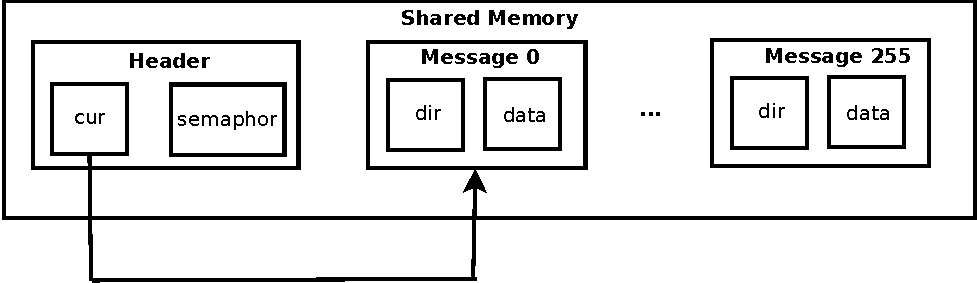
\includegraphics[width=0.75\textwidth]{a4-crop}
\end{figure}

\subsection{Initialisierung: queue\_init}

\texttt{queue\_init} erstellt via \texttt{shm\_open} das Shared Memory-Segment,
setzt die Größe (in Bytes) und bildet es in den Arbeitsspeicher des Programms
ab. Weiterhin wird der Speicherbereich mit Nullen initialisiert und der
Semaphor initialisiert. Da bei einem \texttt{fork} der Arbeitsspeicher nicht
verändert wird, ist die Abbildung des Shared Memory-Segments auch in den
Kindprozessen ohne weitere Initialisierung direkt nutzbar.

\subsection{Schreiben eines neuen Eintrags: queue\_write}

In der Funktion \texttt{queue\_write} wird zunächst via Semaphor die
Datenstruktur gesperrt. Dies ist nötig, damit anschließend deterministisch die
Stelle bestimmt werden kann, an welcher das nächste Element eingefügt wird.
Diese wird dadurch gefunden, dass frisch initialisierte und bereits bearbeitete
Einträge den Wert \texttt{D\_INVALID} als \texttt{dir} (Direction) besitzen.
\np

Nun wird das Element via \texttt{memcpy} kopiert, der \texttt{cur}-Wert im
Header (für das aktuelle Element) angepasst und der Semaphor wieder entsperrt.

\subsection{Richtung des aktuellen Eintrags abrufen}

Die Richtung des aktuellen Eintrags lässt sich sehr einfach herausfinden, indem
das aktuelle Element ermittelt wird und anschließend der \texttt{dir}-Wert
zurückgegeben wird.
\np

Diese Funktion arbeitet ohne Locks oder zusätzliche Variablen auf dem Stack. Da
sie in einer Schleife permanent aufgerufen wird, solange die einzelnen Prozesse
warten, ist dies eine gute Eigenschaft.

\subsection{Daten abrufen und Element invalidieren: queue\_get\_data}

Da durch die Richtung (\texttt{dir}) immer klar ist, von welchem Prozess die
Nachricht kommt und an welchen sie gerichtet ist, ruft immer genau der richtige
Prozess \texttt{queue\_\-get\_\-data} auf, und sonst keiner. Deshalb haben wir uns
entschieden, die Funktion atomar den Datenwert der aktuellen Nachricht
zurückgeben zu lassen und diesen gleichzeitig zu invalidieren.
\np

Die Invalidierung geschieht, indem der \texttt{dir}-Wert auf
\texttt{D\_INVALID} gesetzt und der \texttt{cur}-Wert im Header auf das nächste
Element verschoben wird.


\end{document}
